\usetikzlibrary{calc,decorations.markings}
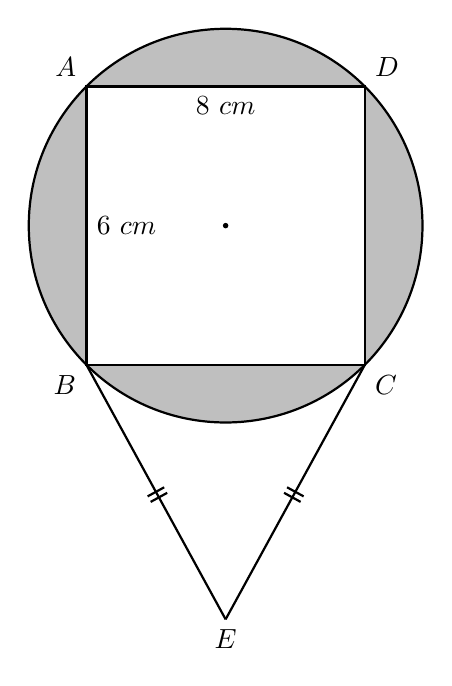
\begin{tikzpicture}[thick,
    double tick mark/.style={
        decoration={markings,
            mark=at position 0.5 with {
                \draw (0,-0.12) -- (0,0.12);
                \draw (0.08,-0.12) -- (0.08,0.12);
            }
        },
        postaction={decorate}
    }
]

% Circle radius
\def\r{2.5}

% Center
\coordinate (O) at (0,0);

% Square vertices using angles on circle
\coordinate (A) at (135:\r);
\coordinate (D) at (45:\r);
\coordinate (B) at (225:\r);
\coordinate (C) at (315:\r);

% Bottom point E
\coordinate (E) at (0, -\r - 2.5);

% --- Fill circular segments with solid grey ---
\fill[gray!50] (O) circle (\r);
\fill[white] (A) -- (D) -- (C) -- (B) -- cycle;

% Draw circle
\draw (O) circle (\r);
\fill (O) circle (1pt);

% Draw square
\draw (A) -- (D) -- (C) -- (B) -- cycle;

% Lines from B and C to E with double equal tick marks
\draw[double tick mark] (B) -- (E);
\draw[double tick mark] (C) -- (E);

% --- Labels ---
% "6 cm" on left side
\node[right] at ($(A)!0.5!(B)$) {$6\ cm$};
\node[below] at ($(A)!0.5!(D)$) {$8\ cm$};

% Vertex labels
\node[above left]  at (A) {$A$};
\node[above right] at (D) {$D$};
\node[below left]  at (B) {$B$};
\node[below right] at (C) {$C$};
\node[below]       at (E) {$E$};

\end{tikzpicture}